\documentclass[tikz,border=10pt]{standalone}
\usetikzlibrary{calc}
\begin{document}
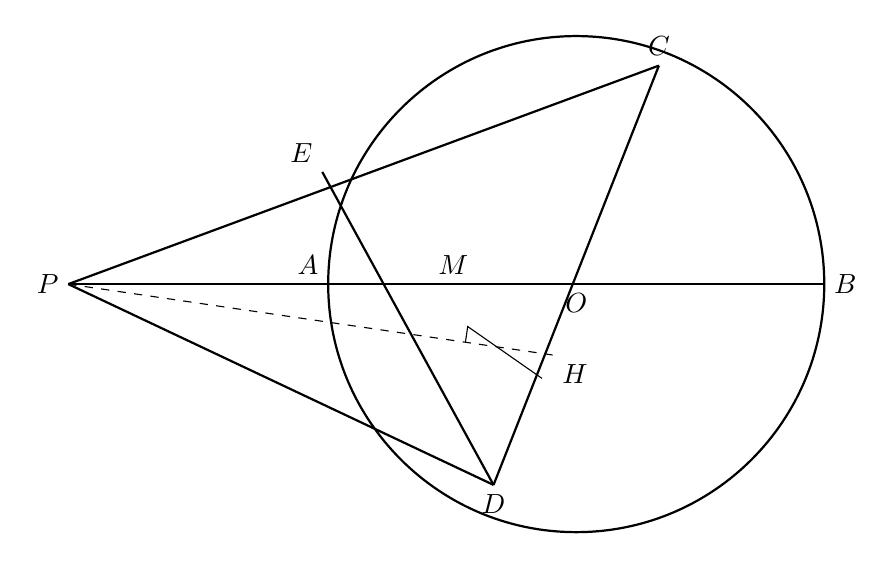
\begin{tikzpicture}[scale=1.5]
\coordinate (P) at (0,0);
\coordinate (A) at (2.2,0);
\coordinate (B) at (6.4,0);
\coordinate (O) at (4.3,0);
\coordinate (M) at (3.05,0);
\coordinate (C) at (5.0,1.85);
\coordinate (D) at (3.6,-1.7);
\coordinate (E) at (2.15,0.95);
\coordinate (H) at (4.1,-0.6);

\draw[thick] (O) circle (2.1);
\draw[thick] (P) -- (B);
\draw[thick] (P) -- (C);
\draw[thick] (P) -- (D);
\draw[thick] (E) -- (D);
\draw[thick] (C) -- (D);

\draw[dashed] (P) -- (H);

% right angle mark at H
\draw ($(H)!0.18!(P)$) -- ($($(H)!0.18!(P)$)!0.18!90:(H)$) -- ($(H)!0.18!(D)$);

\node[left] at (P) {$P$};
\node[above left] at (A) {$A$};
\node[right] at (B) {$B$};
\node[below] at (O) {$O$};
\node[above right] at (M) {$M$};
\node[above] at (C) {$C$};
\node[below] at (D) {$D$};
\node[above left] at (E) {$E$};
\node[below right] at (H) {$H$};
\end{tikzpicture}
\end{document}
